\section{Новая информация о российских примитивах}

В этом разделе обсуждаются последствия того факта, что \(\pi\) является экземпляром TKlog. Сначала утверждается, что наличие структуры TKlog может быть осознанным выбором разработчиков (Раздел 4.1). Затем в Раздел 4.2 вводится новое представление двоичной матрицы, которая используется в алгоритме Стрибог, с помощью которого рассматриваются некоторые взаимодействия между разбиениями, сохраняемыми \(\pi\), и этой линейной компонентой. Наконец, в Разделе 4.3. обсуждаются результаты и их последствия.

\subsection{Вероятный процесс проектирования \(\pi\)}
В свете полученных результатов можно получить некоторую информацию о процессе проектирования \(\pi\). Во-первых, устанавливается, что количество экземпляров TKlog крайне мало, а значит, выбор этой структуры был преднамеренным. Затем, используя некоторые экспериментальные результаты, представляется процесс проектирования, который дает результаты, чрезвычайно похожие на \(\pi\).

\textbf{Плотность множества TKlog.} Помимо высокоуровневого алгоритма, 8-битный TKlog полностью определяется тремя компонентами: примитивным многочленом \(p\) степени $8$ (существует $16$ возможных вариантов), аффинной функцией \(\kappa : x \mapsto \Lambda(x) \oplus \kappa(0)\), где двоичная матрица \(\Lambda\) размера \(8 \times 4\) такая, что \(\Lambda(\mathbb{F}_{2}^{4})\) и \(\text{GF}(2^4)\) лежат в \(\text{GF}(2^8)\), и перестановкой \(s\) над \(\mathbb{Z}/15\mathbb{Z}\). Матрица \(\Lambda\) должна быть такой, чтобы ее первый столбец \(\Lambda_0\) не был элементом \(\text{GF}(2^4)\), второй — не был элементом \(\text{GF}(2^4) \cup (\Lambda_0 \oplus \text{GF}(2^4))\) и т. д., всего для этой матрицы существует существует \((2^8 - 2^4)(2^8 - 2^5)(2^8 - 2^6)(2^8 - 2^7) \approx 2^{30.3}\) вариантов. Таким образом, существует около
\[
  \underbrace{16}_{p} \times \underbrace{2^{30.3}}_{\Lambda} \times \underbrace{2^8}_{\kappa(0)} \times \underbrace{15!}_{s} \approx 2^{82.6}
\]
различных экземпляров 8-битных TKlog.

Это число очень мало. Для сравнения, существует всего \(2^8! \approx 2^{1684}\) перестановок \(\mathbb{F}_2^8\), из которых \(2^8 \times \prod_{i=0}^{7}(2^8 - 2^i) \approx 2^{70.2}\) являются аффинными. Таким образом, число экземпляров TKlog примерно в 4000 раз больше числа аффинных перестановок.

Эти оценки нужны для того, чтобы дать представление о том, насколько мало число экземпляров TKlog. Предполагается, что генератор случайных перестановок, возвращающий аффинную перестановку, будет намеренно генерировать такой объект. Точно так же можно предположить, что процесс генерации, который привел разработчиков Стрибога к выбору \(\pi\), намеренно вернул экземпляр TKlog.

\textbf{Утверждение.} Разработчики \(\pi\) сознательно выбрали эту структуру, учитывая малое число экземпляров TKlog.

\textbf{Экспериментальные результаты.} Насколько хороши разностные и линейные свойства экземпляров TKlog по сравнению с теми, которые ожидаются от случайной перестановки? Ответ на этот вопрос будет основыватся на анализе S-блока Skipjack из \cite{BP15}, также будут введены следующие понятия.

\textbf{Определение 2} \textit{(Аномалия S-блока.)} Пусть \(F : \mathbb{F}_2^n \to \mathbb{F}_2^n\) — перестановка, \(u(F)\) — ее разностная однородность, а \(N_k(F)\) — число вхождений \(k\) в ее DDT. Разностная аномалия \(F\) равна
\[
A_d^F = -\log_2(\mathrm{Pr}[u(G) \leq u(F) \text{ и } N_{u(F)}(G) \leq N_{u(F)}(F)]),
\]
где вероятность берется по всем перестановкам \(G\). Если \(\ell(F)\) — линейность \(F\) и \(N'_k(F)\) — сумма числа вхождений \(k\) и \(-k\) в LAT \(F\), то линейная аномалия \(F\) равна
\[
A_\ell^F = -\log_2(\mathrm{Pr}[\ell(G) \leq \ell(F) \text{ и } N'_{\ell(F)}(G) \leq N'_{\ell(F)}(F)]),
\]
где вероятность берется по всем перестановкам \(G\).

S-блок с разностной аномалией, близкой к 0, имеет разностнык свойства, близкие свойству случайного S-блока или даже хуже. Разностная аномалия ведет себя так, как и ожидалось: при уменьшении значения разностной однородности ниже ожидаемого, значение аномалии возрастает. Поскольку она содержит больше информации, чем разностная однородность, она позволяет сравнивать S-блоки, для которых это значение одинаково. С криптографической точки зрения, чем выше аномалия, тем лучше, так как это означает, что S-блок обеспечит лучшую защиту от разностных атак. То же самое можно сказать о линейной аномалии.

В своей работе \cite{BP15} Бирюков и Перрин предоставили формулы для вычисления разностных и линейных аномалий, основанные на статистическом распределении коэффициентов DDT и LAT, представленных в \cite{DR07}. Они также показали, что линейная аномалия S-блока Skipjack равна 55.4, так что этот компонент не мог быть сгенерирован случайным образом.

Чтобы попытаться собрать больше информации о процессе проектирования \(\pi\), было сгенерировано \(10^6\) случайных 8-битных экземпляров TKlog. Были изображены разностные и линейные аномалии каждого из них на двумерной диаграмме, представленной на Рисунке \ref{fig:fig03}. Каждому экземпляру соответствует светло-серая точка; более темные точки получаются, когда несколько экземпляров имеют одни и те же разностные и линейные аномалии. Также в эту диаграмму были включены аномалии \(\pi\), \(\log^{\text{FLY}}_\alpha\) и \(\log^{\text{HN}}_\alpha\).

\begin{figure}
  \centering
  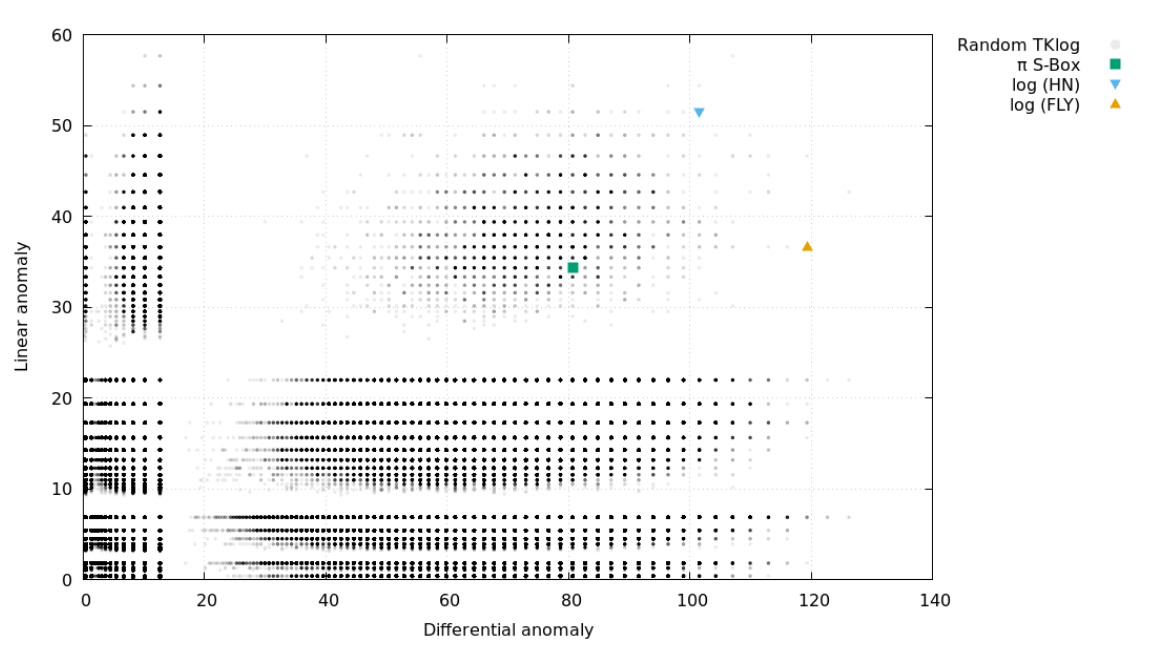
\includegraphics[scale=0.7]{contents/pics/anomalies.png}
  \caption{Разностные и линейные аномалии случайных 8-битных экземпляров TKlog, \(\pi\), \(\log^{\text{FLY}}_\alpha\) и \(\log^{\text{HN}}_\alpha\)}
  \label{fig:fig03}
\end{figure}

Можно заметить, что разностные и линейные аномалии \(\pi\) ''несколько хороши'', но не исключительны относительно аномалий случайного экземпляра TKlog. Точнее, 8-битный TKlog имеет как разностные и линейные аномалии, не ниже, чем у \(\pi\) с вероятностью около \(2^{-10.6}\), и нетрудно получить гораздо лучшие случаи. Они также ниже, чем у \(\log^{\text{FLY}}_\alpha\) и \(\log^{\text{HN}}_\alpha\).

Однако, ни один из полученных случайных экземпляров не имеет лучшей разностной однородности или линейности, чем \(\pi\) (включая \(\log^{\text{FLY}}_\alpha\) и \(\log^{\text{HN}}_\alpha\)). Более того, \(\pi\) находится в области на Рисунке \ref{fig:fig03}, которая содержит большинство экземпляров с той же разностной однородностью и линейностью. Таким образом, аномалии \(\pi\) соответствуют аномалиям случайного экземпляра TKlog с той же разностной однородностью и линейностью.

\textbf{Схема процесса проектирования.} В свете вышеприведенных экспериментальных результатов, можно увидеть, что следующий процесс проектирования приведет к результату, очень похожему на \(\pi\).

\begin{enumerate}
  \item Определить, что наилучшая возможная разностная однородность для 8-битного экземпляра TKlog равна 8, а наилучшая линейность — 56, например, с помощью обширного компьютерного моделирования.
  \item Выбрать случайным образом экземпляр TKlog среди тех, которые обладают указанными выше разностной однородностью и линейностью, не принимая во внимание аномалию.
\end{enumerate}

Эта стратегия естественна до тех пор, пока существует причина навязывать использование TKlog (хотя не получается придумать ни одной). Поскольку  разностные и линейные аномалии \(\pi\) уступают аномалиям \(\log^{\text{FLY}}_\alpha\) и \(\log^{\text{HN}}_\alpha\), целью использования TKlog в данном случае не может быть улучшение криптографических свойств дискретного логарифма. Более того, сильные алгебраические свойства компонентов, описанных в Разделе 2.2, априори требуют осторожности, тем более в случае Стрибога. Действительно, как будет объяснено ниже, его линейный слой нетривиальным образом взаимодействует с соответствующими разбиениями.

\subsection{О линейном слое в Стрибоге}
Бинарная матрица, соответствующая операции L Стрибога, представлена на Рисунке \ref{fig:04}, где черный пиксель соответствует 1, а белый — 0.

\begin{figure}
  \centering
  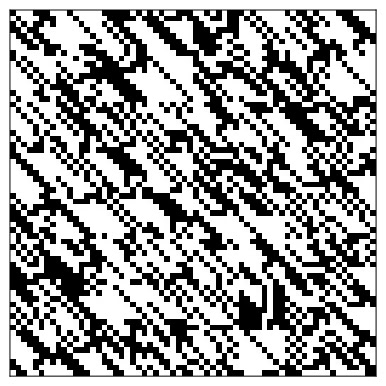
\includegraphics[scale=0.9]{contents/pics/Streebog_matrix.png}
  \caption{Двоичная матрица L \(64 \times 64\), используемая в алгоритме Стрибог}
  \label{fig:04}
\end{figure}

Как можно заметить, матрица имеет сильную структуру. В \cite{KK13} Казимиров и Казимирова показали, что ее можно записать как композицию:
\begin{itemize}
    \item слой 8-битных линейных перестановок \(\ell\), который просто инвертирует порядок битов в каждом байте;
    \item умножение на $8 \times 8$ MDS-матрицу из $GF(2^8) = F_2[X]/P_{KK}(X)$, где \(P_{KK}(X) = X^8 \oplus X^6 \oplus X^5 \oplus X^4 \oplus 1\) — примитивный многочлен степени 8;
    \item величина, обратная слою \(\ell\).
\end{itemize}

В данной работе использовался прямой подход для упрощения этой структуры: каждый байт в строке устанавливался равным 1 по очереди, умножая его на L, затем записывались байты как элементы $GF(2^8) = F_2[X]/p_{\text{min}}(X)$, генерируя матрицу $L^F$ такую следующего вида:
\begin{figure}
  \centering
  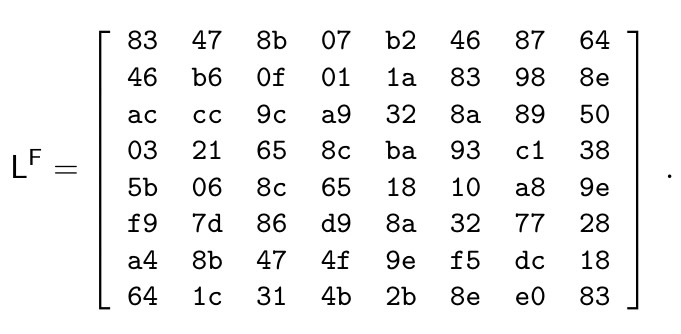
\includegraphics[scale=0.9]{contents/pics/LF_matrix.png}
\end{figure}

Многочлен, используемый Казимировым и Казимировой, является обратным \(p_{\text{min}}\), т.е. \(P_{KK}(1/X) = p_{\text{min}}(X)/X^8\). Оглядываясь назад, очевидно, что, используя этот многочлен, можно устранить обратный порядок бит в байте в представлении ими линейного слоя.

В итоге, если обозначить как $A$ матрицу размера $8 \times 8$, состоящую из элементов из $GF(2^8)$, соответствующую внутреннему состоянию Стрибога, и как P транспонированную матрицу $A$ (как указано в спецификации Стрибог), то применение всей линейной части раундовой функции Стрибог можно записать в виде
\[
(L \circ P)(A) = A^T \times L^F,
\]
где ''$\times$'' обозначает обычное умножение матриц.

\textbf{Аддитивные и мультипликативные смежные классы.} Подполе $GF(2^4)^*$ имеет особую связь с $L$. Действительно, применение умножения матрицы Стрибога к вектору \(x_i = [0, \ldots, 0, x, 0, \ldots, 0]\) из $GF(2^8)^8$, так, что \(x_i^i = x\) и \(x_i^k = 0\), при \(k \neq i\), эквивалентно вычислению
\[
v = x^i \times L^F = [L^F_{i,0} \odot x, ..., L^F_{i,7} \odot x],
\]
так, что если \(x \in GF(2^m)^*\), то \(v_j \in LF_{i,j} \cdot GF(2^m)^*\), т.е., оно отображает подполе на его мультипликативные смежные классы. Однако, непонятно, что происходит, когда активны несколько ячеек входного вектора.

\textbf{Кузнечик.} Линейный слой Кузнечика определяется как LFSR с $16$ ячейками, каждая из которых является элементом $GF(2^8)$, и который сдвигается на $16$ тактов. Его также можно представить как умножение на матрицу размером $16 \times 16$. Однако, для представления элементов поля используется другой многочлен, а именно \(p_{\text{kuz}}(X) = X^8 \oplus X^7 \oplus X^6 \oplus X \oplus 1\). Если \(p_{\text{min}}(X) = X^8 \oplus X^4 \oplus X^3 \oplus X^2 \oplus 1\) является первым примитивным многочленом степени $8$, записанным в лексикографическом порядке, то \(p_{\text{kuz}}\) — последний такой многочлен веса $5$, как указано в \cite{LN97}.

В отличие от умножения на матрицу в Стрибоге, в Кузнечике его нельзя записать как матричное умножение в $F_2[X]/p_{\text{min}}(X)$, так что распространение классов смежности, описанное выше для хеш-функции, не применимо к блочному шифру.

\subsection{Обсуждение}

Последствия сохранения разбиения на смежные классы \(\pi\) и его нетривиального взаимодействия с линейным слоем оценить сложно.

В литературе можно найти другие S-блоки, отображающие смежные классы в смежные классы. Например, мономы отображают мультипликативные смежные классы подполя в мультипликативные смежные классы подполя: если \(F: x \mapsto x^d\) является перестановкой над $GF(2^{2m})$, то
\[
F(\alpha^i \cdot GF(2^m)) = \alpha^{d \times i} \odot GF(2^m).
\]

Если убрать их аффинные компоненты, то S-блоки AES \cite{AES01} и Misty1 \cite{Mat97} (среди многих других) демонстрируют такое поведение. Тем не менее, несмотря на их появление в некоторых очень известных целях, мультипликативные смежные классы никогда не использовались в симметричном криптоанализе. Стоит заметить, что разработчики алгоритмов всегда сочетают обратные функции с несвязанными аффинными слоями, чтобы разрушить его алгебраическую структуру. Это консервативное решение, вероятно, предназначено для предотвращения использования мультипликативных смежных классов атак на эти шифры на практике.

Это не так с аддитивными смежными классами. На самом деле, авторы работы \cite{BBF16} намеренно построили S-блок, отображающий аддитивные смежные классы в аддитивные смежные классы, с явной целью использовать этот шаблон в качестве бэкдора. Они показывают, что такое разбиение может быть сохранено при тщательном выборе линейного слоя и может сохраняться в течение произвольного количества раундов. Причина, по которой Bannier и другие рассматривали аддитивные смежные классы, заключается в следующем наблюдении.

\textit{Примечание 1.} Если \(F_k: x \mapsto x \oplus k\) — добавление ключа в $F^n_2$, и \(V\) — векторное подпространство $F^n_2$, тогда
\[
F_k(c \oplus V) = (k \oplus c) \oplus V,
\]
так, что разбиение $F^n_2$ на аддитивные смежные классы \(V\) сохраняется под действием \(F_k\) независимо от \(k\).

В шифре Bannier и др., ключевое расписание может быть произвольно сложным, не препятствуя работе бэкдора. Это свойство не распространяется на разбиение на мультипликативные смежные классы.

Единственным случай (кроме TKlog), когда разбиение на смежные классы отображактся на другое разбиение, являются дискретные логарифмы. Действительно, логарифм типа Hakala-Nyberg, действующий на $GF(2^{2m})$, который отображает \(\alpha^{2^m-1}\) в $0$, всегда отображает мультипликативные смежные классы подполя на аддитивные смежные классы $\mathbb{Z}/(2^m - 1)\mathbb{Z}$. В этом случае умножение производится в конечном поле, а сложение с целыми числами. Поскольку эти две операции совершенно разные, маловероятно, что эта характеристика помогает в криптоанализе.

В итоге, рассматривая влияние смежных классов на симметричные примитивы, получается одна из следующих ситуаций:
\begin{enumerate}
    \item разбиение на смежные классы не может быть итеративным, поскольку входное и выходное разбиения находятся в совершенно разных структурах (случай логарифма);
    \item хотя S-блок и линейный слой определены над схожими структурами, была добавлена небольшая функция с явной целью нарушить это сходство (случай AES и аффинной перестановки, использованной в S-блоке);
    \item S-блок и линейный слой были выбраны с выровненными структурами, которые сохраняют одно и то же разбиение, чтобы целенаправленно внедрить бэкдор в блочном шифре \cite{BBF16}.
\end{enumerate}

По-видимому, Кузнечик относится ко второму случаю. Несмотря на то, что разработчики не предоставили свой анализа безопасности, было бы логично, чтобы они выбрали многочлен, используемый для определения конечного поля, в котором функционирует линейный слой, чтобы не 'выравнивать' его со структурой, используемой для построения \(\pi\).

Однако Стрибог не подпадает ни в одну из этих категорий. Входные и выходные смежные классы определены над той же структурой (конечным полем), поэтому он не относится к первой ситуации. S-блок мог быть составлен с аффинным слоем, нарушающим связь с $GF(2^8)$ (как в AES), или линейный слой мог быть определен над другим конечным полем (как в Кузнечике), но ни того, ни другого не происходит, поэтому он не подпадает и под вторую категорию. Тем не менее, хотя линейный слой определен над той же структурой, что и смежные классы, сохраняемые S-блоком, эти разбиения отличаются, и неясно, как они могут взаимодействовать с матричным умножением. Поэтому не является очевидным тот факт, что Стрибог относится к третьей категории, и следующая проблема остается открытой.

\textbf{Открытая проблема 1.} Существует ли способ использовать сохранение разбиения \(\pi\) для атаки на Стрибог?